% Concept figures shared by the specifications, taken unchanged from the IEEE Trans. IT paper (papers/WLZ.pdf):
% Figures 1 (parsers), 2 (indexes) and its multi-window parse example (mwparse)
\documentclass[tikz,border=8pt]{standalone}
\usepackage{amsmath,amssymb}
\usepackage{xcolor}
\pagecolor{white}
\usetikzlibrary{decorations.pathreplacing}
\begin{document}

%% 1. parsers
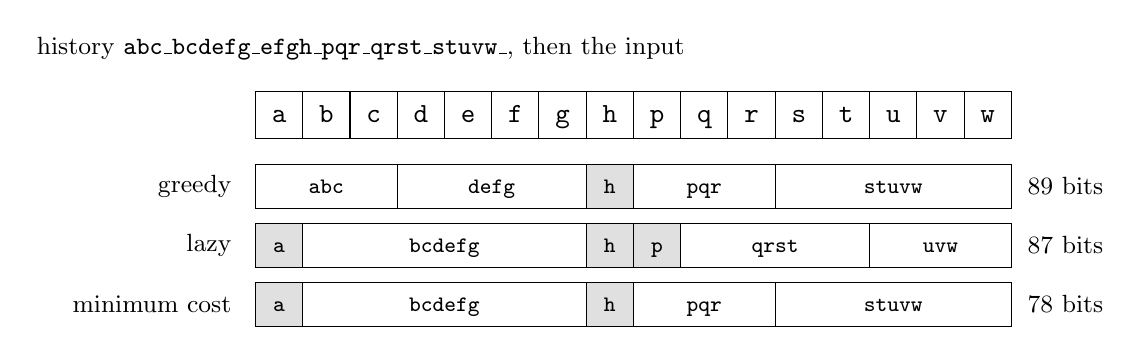
\begin{tikzpicture}[font=\small,
  cell/.style={draw, minimum width=6mm, minimum height=6mm, inner sep=0pt, font=\ttfamily,
    text height=1.6ex, text depth=0.3ex},
  lit/.style={draw, fill=black!12},
  mat/.style={draw},
  row/.style={anchor=east, inner sep=0pt},
  cost/.style={anchor=west, inner sep=0pt}]
\node[anchor=west] at (-2.6,0.85) {history \texttt{abc\_bcdefg\_efgh\_pqr\_qrst\_stuvw\_}, then the input};
\foreach \c [count=\i] in {a,b,c,d,e,f,g,h,p,q,r,s,t,u,v,w}
  \node[cell] at (0.6*\i,0) {\c};
\newcommand{\phr}[5]{\draw[#5] (0.6*#2-0.3,#1-0.28) rectangle (0.6*#2+0.6*#3-0.3,#1+0.28);
  \node[font=\ttfamily\footnotesize, text height=1.5ex, text depth=0.3ex] at (0.6*#2+0.3*#3-0.3,#1) {#4};}
\node[row] at (0.0,-0.9) {greedy};
\phr{-0.9}{1}{3}{abc}{mat} \phr{-0.9}{4}{4}{defg}{mat} \phr{-0.9}{8}{1}{h}{lit}
\phr{-0.9}{9}{3}{pqr}{mat} \phr{-0.9}{12}{5}{stuvw}{mat}
\node[cost] at (10.1,-0.9) {89 bits};
\node[row] at (0.0,-1.65) {lazy};
\phr{-1.65}{1}{1}{a}{lit} \phr{-1.65}{2}{6}{bcdefg}{mat} \phr{-1.65}{8}{1}{h}{lit}
\phr{-1.65}{9}{1}{p}{lit} \phr{-1.65}{10}{4}{qrst}{mat} \phr{-1.65}{14}{3}{uvw}{mat}
\node[cost] at (10.1,-1.65) {87 bits};
\node[row] at (0.0,-2.4) {minimum cost};
\phr{-2.4}{1}{1}{a}{lit} \phr{-2.4}{2}{6}{bcdefg}{mat} \phr{-2.4}{8}{1}{h}{lit}
\phr{-2.4}{9}{3}{pqr}{mat} \phr{-2.4}{12}{5}{stuvw}{mat}
\node[cost] at (10.1,-2.4) {78 bits};
\end{tikzpicture}

%% 2. indexes
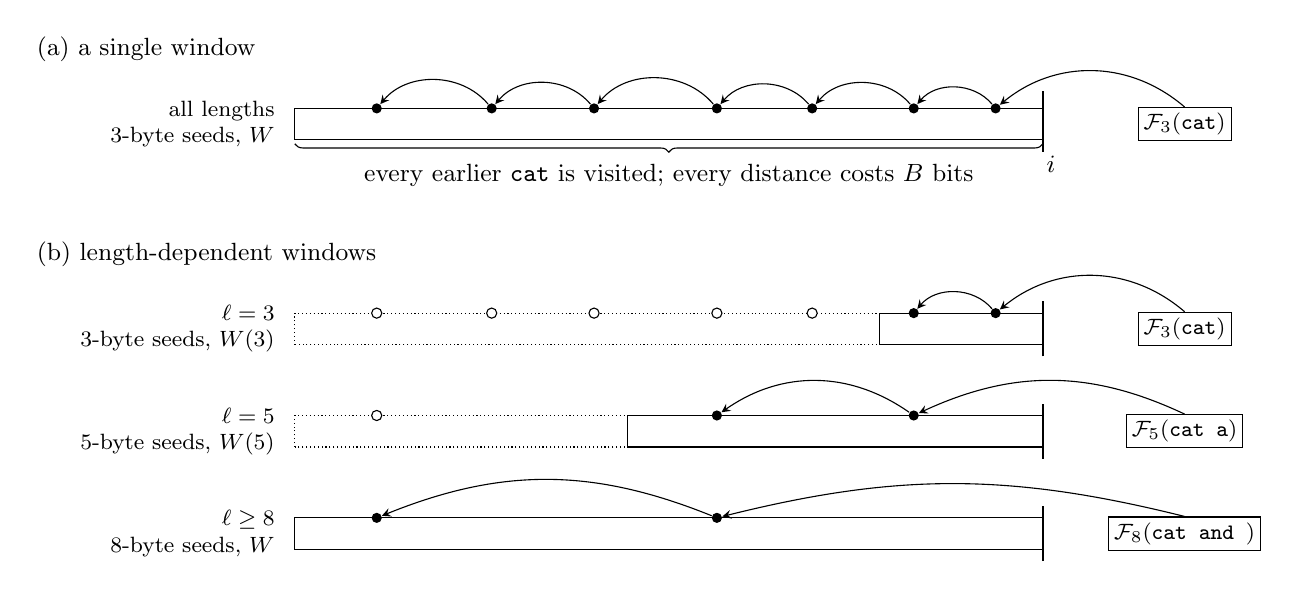
\begin{tikzpicture}[font=\small, >=stealth,
  occ/.style={circle, fill, inner sep=1.3pt},
  far/.style={circle, draw, fill=white, inner sep=1.3pt},
  head/.style={draw, inner sep=2pt, font=\footnotesize},
  lab/.style={anchor=east, align=right, inner sep=0pt, font=\footnotesize},
  brc/.style={decorate, decoration={brace, mirror, amplitude=3pt}},
  chain/.style={->, bend right=50}]
\node[anchor=west] at (-3.4,1.15) {(a) a single window};
\node[lab] at (-0.25,0.2) {all lengths\\3-byte seeds, $W$};
\draw (0,0) rectangle (9.5,0.4);
\draw[thick] (9.5,-0.15) node[below right, inner sep=1pt] {$i$} -- (9.5,0.62);
\foreach \x [count=\k] in {8.9,7.86,6.57,5.36,3.8,2.5,1.04} \node[occ] (a\k) at (\x,0.4) {};
\node[head] (ha) at (11.3,0.2) {$\mathcal F_3(\texttt{cat})$};
\draw[->] (ha.north) to[bend right=40] (a1);
\foreach \k [evaluate=\k as \n using int(\k+1)] in {1,...,6} \draw[chain] (a\k) to (a\n);
\draw[brc] (0,-0.05) -- (9.5,-0.05) node[midway, below=4pt]
  {every earlier \texttt{cat} is visited; every distance costs $B$ bits};
\node[anchor=west] at (-3.4,-1.45) {(b) length-dependent windows};
\node[lab] at (-0.25,-2.4) {$\ell=3$\\3-byte seeds, $W(3)$};
\draw[densely dotted] (0,-2.6) rectangle (7.43,-2.2);
\draw (7.43,-2.6) rectangle (9.5,-2.2);
\draw[thick] (9.5,-2.75) -- (9.5,-2.05);
\node[occ] (b1) at (8.9,-2.2) {}; \node[occ] (b2) at (7.86,-2.2) {};
\foreach \x in {6.57,5.36,3.8,2.5,1.04} \node[far] at (\x,-2.2) {};
\node[head] (hb) at (11.3,-2.4) {$\mathcal F_3(\texttt{cat})$};
\draw[->] (hb.north) to[bend right=40] (b1);
\draw[chain] (b1) to (b2);
\node[lab] at (-0.25,-3.7) {$\ell=5$\\5-byte seeds, $W(5)$};
\draw[densely dotted] (0,-3.9) rectangle (4.23,-3.5);
\draw (4.23,-3.9) rectangle (9.5,-3.5);
\draw[thick] (9.5,-4.05) -- (9.5,-3.35);
\node[occ] (c1) at (7.86,-3.5) {}; \node[occ] (c2) at (5.36,-3.5) {};
\node[far] at (1.04,-3.5) {};
\node[head] (hc) at (11.3,-3.7) {$\mathcal F_5(\texttt{cat\ a})$};
\draw[->] (hc.north) to[bend right=25] (c1);
\draw[->, bend right=35] (c1) to (c2);
\node[lab] at (-0.25,-5.0) {$\ell\ge8$\\8-byte seeds, $W$};
\draw (0,-5.2) rectangle (9.5,-4.8);
\draw[thick] (9.5,-5.35) -- (9.5,-4.65);
\node[occ] (d1) at (5.36,-4.8) {}; \node[occ] (d2) at (1.04,-4.8) {};
\node[head] (hd) at (11.3,-5.0) {$\mathcal F_8(\texttt{cat\ and\ })$};
\draw[->] (hd.north) to[bend right=14] (d1);
\draw[->, bend right=22] (d1) to (d2);
\end{tikzpicture}

%% 3. mwparse
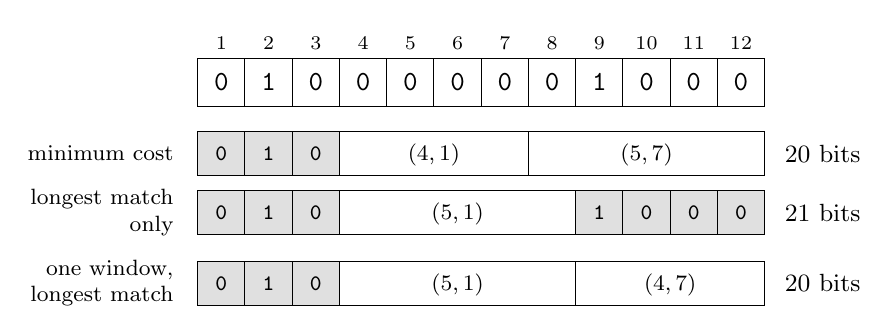
\begin{tikzpicture}[font=\small,
  cell/.style={draw, minimum width=6mm, minimum height=6mm, inner sep=0pt, font=\ttfamily,
    text height=1.6ex, text depth=0.3ex},
  lit/.style={draw, fill=black!12},
  mat/.style={draw},
  row/.style={anchor=east, inner sep=0pt, align=right, font=\footnotesize},
  cost/.style={anchor=west, inner sep=0pt}]
\foreach \c [count=\i] in {0,1,0,0,0,0,0,0,1,0,0,0} {
  \node[cell] at (0.6*\i,0) {\c};
  \node[font=\scriptsize] at (0.6*\i,0.5) {\i};}
\newcommand{\phr}[5]{\draw[#5] (0.6*#2-0.3,#1-0.28) rectangle (0.6*#2+0.6*#3-0.3,#1+0.28);
  \node[font=\footnotesize, text height=1.5ex, text depth=0.3ex] at (0.6*#2+0.3*#3-0.3,#1) {#4};}
\node[row] at (0.0,-0.9) {minimum cost};
\phr{-0.9}{1}{1}{\texttt{0}}{lit} \phr{-0.9}{2}{1}{\texttt{1}}{lit} \phr{-0.9}{3}{1}{\texttt{0}}{lit}
\phr{-0.9}{4}{4}{$(4,1)$}{mat} \phr{-0.9}{8}{5}{$(5,7)$}{mat}
\node[cost] at (7.75,-0.9) {20 bits};
\node[row] at (0.0,-1.65) {longest match\\only};
\phr{-1.65}{1}{1}{\texttt{0}}{lit} \phr{-1.65}{2}{1}{\texttt{1}}{lit} \phr{-1.65}{3}{1}{\texttt{0}}{lit}
\phr{-1.65}{4}{5}{$(5,1)$}{mat}
\phr{-1.65}{9}{1}{\texttt{1}}{lit} \phr{-1.65}{10}{1}{\texttt{0}}{lit}
\phr{-1.65}{11}{1}{\texttt{0}}{lit} \phr{-1.65}{12}{1}{\texttt{0}}{lit}
\node[cost] at (7.75,-1.65) {21 bits};
\node[row] at (0.0,-2.55) {one window,\\longest match};
\phr{-2.55}{1}{1}{\texttt{0}}{lit} \phr{-2.55}{2}{1}{\texttt{1}}{lit} \phr{-2.55}{3}{1}{\texttt{0}}{lit}
\phr{-2.55}{4}{5}{$(5,1)$}{mat} \phr{-2.55}{9}{4}{$(4,7)$}{mat}
\node[cost] at (7.75,-2.55) {20 bits};
\end{tikzpicture}

\end{document}
